\section{Electronics and Data Acquisition}
\label{sec:daq}
The SK Electronics and Data Acquisition System (DAQ) was extensively upgraded between SK-III and SK-IV.  As such, the SK-IV electronics will be explained separately from the SK I-III electronics.
\subsection{SK I-III}
\label{subsec:sk_1_3_daq}
The SK I-III DAQ processed ID PMT signals using custom build Analog-Timing-Modules (ATMs), which were originally designed and built by KEK.   A schematic of the ATM can be seen in \cref{fig:daq_ATM}  The PMT signal was split into four signals.  One of these signals was sent to a discriminator, which compared the signal to a threshold corresponding to 1/4 pe equivalent.  When the signal crossed this threshold, a 200ns wide logic pulse was sent to a hardware trigger module.  Simultaneously, the signal from the PMT was stored by a Charge-to-Analog Converter (QAC), and a integration of a constant current was started by a Time-to-Analog Converter (TAC).  When a global trigger was received from the hardware trigger module, the TAC integration was stopped and the information in the QAC and TAC were sent to and Analog-to-Digital Converter (ADC) to be digitized and stored in internal memory.  Because the TAC integrated a constant charge from the time of the channel trigger to the time of the global trigger, the time of the PMT signal relative to the global trigger can be calculated from the total integrated charge on the TAC.  Each channel was assigned two TACs and QACs, in order to process events which might occur in rapid succession, such as the a decay electron following a muon.\par
A hitsum was calculated by the hardware trigger module by simple analog sum of the logic signals from the ATMs.  When the hitsum crossed a given threshold, a global trigger would be issued to the ATMs.  Three different triggers were used: high energy (HE), low energy (LE) and super low energy (SLE).  The HE and LE triggers were set at 31 and 29 hits, respectively, with the LE threshold corresponding to an electron energy of 5.7 MeV.  The SLE trigger was added to lower the energy threshold to 4.6 MeV.  The trigger logic and interaction with the ATMs is shown in \cref{fig:daq_trigger_1_3}, and a full schematic of the DAQ is shown in         

\begin{figure}
\centering
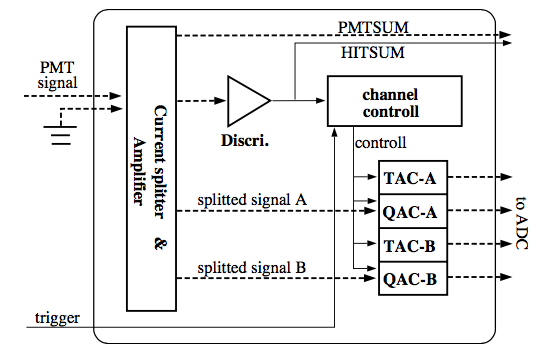
\includegraphics[width=0.8\textwidth]{figures/SK_1_3_ATM.png}
\caption{Schematic of processing of one channel by the ATM, used in SK I-III.  Dashed lines represent analog signals while solid lines represent logic signals \cite{Fukuda:2002uc}.}
\label{fig:daq_ATM}
\end{figure}

\begin{figure}
\centering
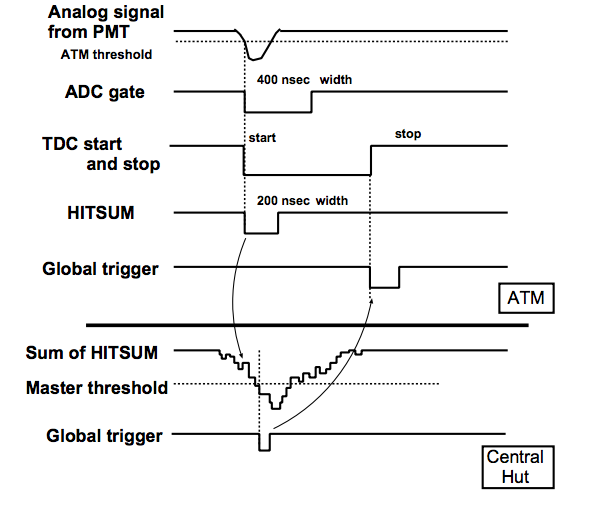
\includegraphics[width=0.8\textwidth]{figures/ID_trigger_SK1_3_Nishino.png}
\caption{Trigger system used in SK I-III \cite{Nishino:2009lps}.}
\label{fig:daq_trigger_1_3}
\end{figure}

\begin{figure}
\centering
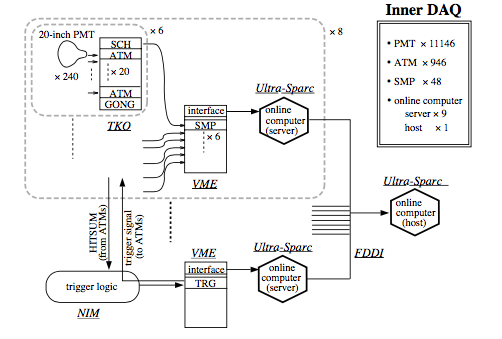
\includegraphics[width=0.8\textwidth]{figures/SK_1_3_daq.png}
\caption{Schematic of SK I-III DAQ.  Lines indicate flow of data \cite{Fukuda:2002uc}.}
\label{fig:daq_trigger_1_3}
\end{figure}

